\documentclass[14pt]{extreport}
\usepackage{cmap}
\usepackage[utf8]{inputenc}
\usepackage[english,ukrainian]{babel}
\usepackage{graphicx}
\usepackage{geometry}
\usepackage{listings}
\usepackage{amsmath}
\usepackage{float}
\geometry{
	a4paper,
	left=20mm,
	right=20mm,
	top=20mm,
	bottom=20mm
}
\lstset{
	language=bash,
	tabsize=4,
	breaklines,
	keepspaces,
	showstringspaces=false,
}
\graphicspath{ {./pictures} }
\setlength{\parindent}{4em}

\newcommand\subject{Кросплатформне програмування}
\newcommand\lecturer{доцент кафедри ПЗ\\Дяконюк Л.М.}
\newcommand\teacher{ст. викл. кафедри ПЗ\\Шкраб Р.Р.}
\newcommand\mygroup{ПЗ-32}
\newcommand\lab{4}
\newcommand\theme{Робота з колекціями}
\newcommand\purpose{Навчитися працювати з колекціями}

\begin{document}
\begin{normalsize}
	\begin{titlepage}
		\thispagestyle{empty}
		\begin{center}
			\textbf{МІНІСТЕРСТВО ОСВІТИ І НАУКИ УКРАЇНИ\\
				НАЦІОНАЛЬНИЙ УНІВЕРСИТЕТ "ЛЬВІВСЬКА ПОЛІТЕХНІКА"}
		\end{center}
		\begin{flushright}
			Інститут \textbf{КНІТ}\\
			Кафедра \textbf{ПЗ}
		\end{flushright}
		\vspace{160pt}
		\begin{center}
			\textbf{ЗВІТ}\\
			\vspace{10pt}
			До лабораторної роботи № \lab\\
			\textbf{На тему}: “\textit{\theme}”\\
			\textbf{З дисципліни}: “\subject”
		\end{center}
		\vspace{40pt}
		\begin{flushright}
			
			\textbf{Лектор}:\\
			\lecturer\\
			\vspace{10pt}
			\textbf{Виконав}:\\
			
			студент групи \mygroup\\
			Коваленко Д.М.\\
			\vspace{10pt}
			\textbf{Прийняв}:\\
			
			\teacher\\
			
			\vspace{28pt}
			«\rule{1cm}{0.15mm}» \rule{1.5cm}{0.15mm} 2023 р.\\
			$\sum$ = \rule{1cm}{0.15mm}……………\\
			
		\end{flushright}
		\vspace{\fill}
		\begin{center}
			\textbf{Львів — 2023}
		\end{center}
	\end{titlepage}
		
	\begin{description}
		\item[Тема.] \theme.
		\item[Мета.] \purpose.
	\end{description}
	

	\section*{Лабораторне завдання}
	6.Завдання: Розробіть систему для планування та управління робочими завданнями та проектами з урахуванням дедлайнів та графіка виконання. Система повинна дозволяти користувачам створювати завдання, призначати їх на конкретні дати та часи, визначати дедлайни, враховувати залежності між завданнями, і відстежувати стан виконання проектів.
	
	
	Додаткові умови:
	\begin{itemize}
		\item Забезпечте можливість створення іерархії завдань, де одне завдання може включати підзавдання.
		\item Реалізуйте календарні та графічні представлення графіків виконання завдань та проектів.
		\item Дозвольте користувачам встановлювати пріоритети завдань та автоматично визначати найважливіші завдання для виконання.
		\item Забезпечте можливість нагадувань та сповіщень про наближення дедлайнів.
		\item Реалізуйте можливість зберігання та відновлення завдань та проектів для подальшого використання.
	\end{itemize}
	\section*{Хід роботи}

	\textbf{\textit{Main.java}}
	\begin{lstlisting}
import java.time.LocalDate;
import java.time.format.DateTimeFormatter;
import java.util.ArrayList;
import java.util.List;
import java.util.Scanner;

public class Main {
	public static void main(String[] args) throws Exception {
		var projects = new ArrayList<Project>();
		var help = "addTask/addProject/list/exit";
		
		Scanner scanner = new Scanner(System.in);
		System.out.println(help);
		
		while (true) {
			var input = scanner.nextLine();
			
			if (input.equalsIgnoreCase("addTask")) {
				System.out.println("Creating new task:");
				System.out.print("\tname: ");
				var name = scanner.nextLine();
				System.out.print("\tdescription: ");
				var description = scanner.nextLine();
				System.out.print("\tdeadline: ");
				var deadline = scanner.nextLine();
				System.out.print("\tpriority: ");
				var priority = scanner.nextLine();
				var task = new Task(deadline, priority, name, description);
				System.out.print("\tadd to: ");
				var taskName = scanner.nextLine();
				var project = findProject(taskName, projects);
				System.out.println(project);
				var inner = findInnerTask(taskName, projects);
				System.out.println(inner);
				if (project != null) {
					project.addTask(task);
				} else if (inner != null) {
					inner.addInnerTask(task);
				} else {
					System.out.println("Cannot add task");
				}
			} else if (input.equalsIgnoreCase("addProject")) {
				System.out.println("Creating new project:");
				System.out.print("\tname: ");
				var name = scanner.nextLine();
				System.out.print("\tdescription: ");
				var description = scanner.nextLine();
				System.out.print("\tdeadline: ");
				var deadline = scanner.nextLine();
				var project = new Project(deadline, name, description);
				projects.add(project);
				System.out.print("Added new project: " + project);
			} else if (input.equalsIgnoreCase("list")) {
				for (var p : projects) {
					System.out.println(p);
				}
			} else if (input.equalsIgnoreCase("exit")) {
				break;
			}
		}
	}
	
	static Project findProject(String name, ArrayList<Project> projects) {
		for (var p : projects) {
			if (p.getName().equalsIgnoreCase(name)) {
				return p;
			}
		}
		return null;
	}
	static Task findInnerTask(String name, ArrayList<Project> projects) {
		for (var p : projects) {
			for (var t : p.tasks) {
				if (t.getName().equalsIgnoreCase(name)) {
					return t;
				}
				var inner = t.findInnerTask(name);
				if (inner != null) {
					return inner;
				}
			}
		}
		return null;
	}
}

enum Priority {
	High,
	Medium,
	Low;
	
	@Override
	public String toString() {
		return switch (this) {
			case High -> "High";
			case Medium -> "Medium";
			case Low -> "Low";
		};
	}
}

class Project {
	Deadline deadline;
	List<Task> tasks;
	String name;
	String description;
	Project(String deadline, String name, String description) {
		this.tasks = new ArrayList<>();
		this.deadline = new Deadline(deadline);
		this.name = name;
		this.description = description;
	}
	Deadline getDeadline() {
		Deadline deadline = null;
		for (var task : this.tasks) {
			if (deadline == null) {
				deadline = task.getDeadline();
			}
			if (task.getDeadline().compareTo(deadline) > 0) {
				deadline = task.getDeadline();
			}
		}
		return this.deadline;
	}
	String getName() {
		return this.name;
	}
	String getDescription() {
		return this.description;
	}
	void addTask(Task task) throws Exception {
		if (task.getDeadline().compareTo(getDeadline()) > 0) {
			throw new Exception("Invalid deadline");
		}
		this.tasks.add(task);
	}
	@Override
	public String toString() {
		StringBuilder format = new StringBuilder();
		format.append("[P] ").append(getName()).append(" - ").append(getDescription()).append(" (Due ").append(getDeadline()).append(")\n");
		for (var task : this.tasks) {
			format.append("\t").append(task).append("\n");
		}
		return format.toString();
	}
}

class Task {
	Deadline deadline;
	Priority priority;
	List<Task> innerTasks;
	String name;
	String description;
	Task(String deadline, String priority, String name, String description) {
		this.deadline = new Deadline(deadline);
		if (priority.equalsIgnoreCase("low")) {
			this.priority = Priority.Low;
		} else if (priority.equalsIgnoreCase("medium")) {
			this.priority = Priority.Medium;
		} else if (priority.equalsIgnoreCase("high")) {
			this.priority = Priority.High;
		}
		this.innerTasks = new ArrayList<>();
		this.name = name;
		this.description = description;
	}
	Task findInnerTask(String name) {
		for (var t : getInnerTasks()) {
			if (t.getName().equalsIgnoreCase(name)) {
				return t;
			}
			var inner = t.findInnerTask(name);
			if (inner != null) {
				return inner;
			}
		}
		return null;
	}
	Deadline getDeadline() {
		var innerTasksDeadline = this.getInnerTasksDeadline();
		if (this.deadline.compareTo(innerTasksDeadline) > 0) {
			return this.deadline;
		} else {
			return innerTasksDeadline;
		}
	}
	Deadline getInnerTasksDeadline() {
		Deadline deadline = this.deadline;
		for (var task : this.innerTasks) {
			if (task.getDeadline().compareTo(deadline) > 0) {
				deadline = task.getDeadline();
			}
		}
		return this.deadline;
	}
	Priority getPriority() {
		return this.priority;
	}
	String getName() {
		return this.name;
	}
	String getDescription() {
		return this.description;
	}
	List<Task> getInnerTasks() {
		return this.innerTasks;
	}
	void addInnerTask(Task task) throws Exception {
		if (task.getDeadline().compareTo(getDeadline()) > 0) {
			throw new Exception("Invalid deadline");
		}
		this.innerTasks.add(task);
	}
	@Override
	public String toString() {
		return this.toString(2);
	}
	String toString(Integer i) {
		StringBuilder format = new StringBuilder();
		format.append("[T]").append(" <").append(getPriority()).append("> ").append(getName()).append(" (Due ").append(getDeadline()).append(")");
		if (!getInnerTasks().isEmpty()) {
			for (var task : this.getInnerTasks()) {
				format.append("\n").append(repeat(i, "\t")).append(task.toString(i + 1));
			}
		}
		return format.toString();
	}
	public static String repeat(int count, String with) {
		return new String(new char[count]).replace("\0", with);
	}
}

class Deadline implements Comparable<Deadline> {
	LocalDate date;
	Deadline(String str) {
		DateTimeFormatter formatter = DateTimeFormatter.ofPattern("yyyy-MM-dd");
		this.date = LocalDate.parse(str, formatter);
	}
	@Override
	public String toString() {
		DateTimeFormatter formatter = DateTimeFormatter.ofPattern("yyyy-MM-dd");
		return this.date.format(formatter);
	}
	@Override
	public int compareTo(Deadline other) {
		return this.date.compareTo(other.date);
	}
}
	\end{lstlisting}	
	
	\begin{figure}[H]
		\centering
		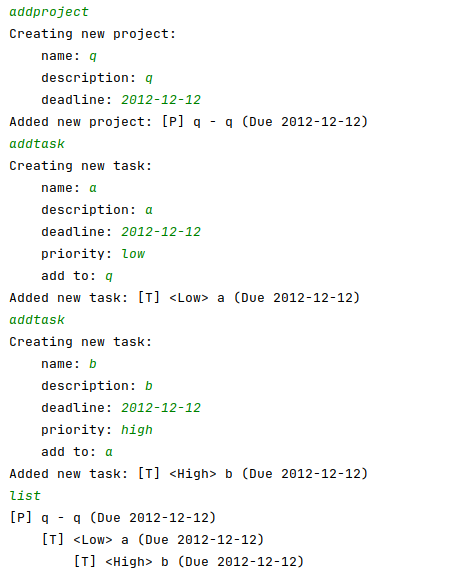
\includegraphics[scale=0.55]{1}
		\caption{Робота програми}
	\end{figure}

	\section*{Висновок}
	Під час виконання лабораторної роботи я працював з колекціями. Навчився працювати з колекціями. Визначив різницю між колекціями.
	 
\end{normalsize}
\end{document}
